\chapter{基于TKEM的协议具体实现与性能评估}\label{chap:implemention}
在本节将介绍如何基于现有的KEM方案实现TKEM，同时阐述如何在原有的协议libsignal框架下引入国密SM系列算法。
\section{基于mlkem和aigis-enc的TKEM方案实现}
目前libsignal在双棘轮阶段采用mlkem来引入会话密钥的抗量子安全性。所以我们首先选择基于Rust实现的mlkem源代码库libcrux来实现TKEM的扩展；其次，在国产的后量子密钥封装算法中选择基于C语言实现的Aigis-Enc代码库进行扩展，然后封装为Rust代码库，最后融入我们的协议实现中。另外，由于目前国产SM系列并没有相关Rust的实现，为了融入国产SM系列算法，将基于由C语言实现的GMSSL代码进行封装，从而提供对应的Rust依赖包。
协议整体实现架构如下所示：
\begin{figure}[htbp]
  \centering
  
    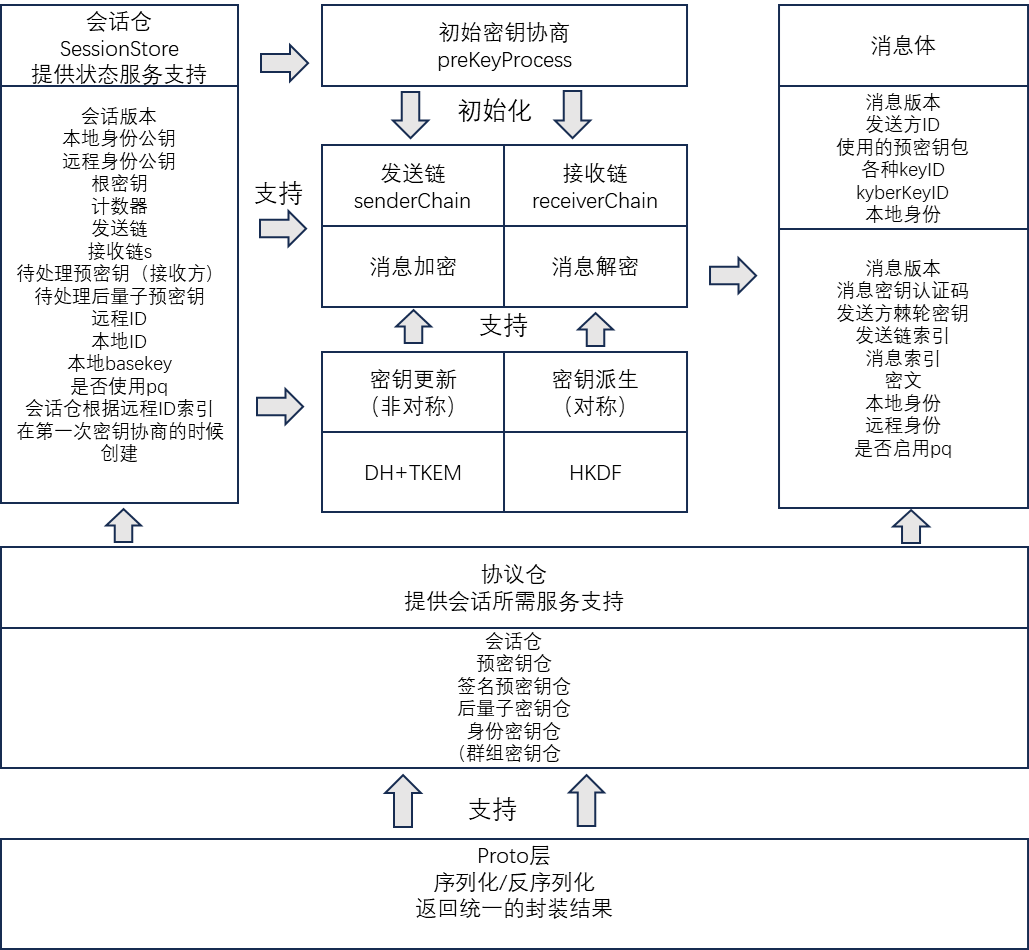
\includegraphics[width=0.9\linewidth]{Img/架构模型.png} 
    \caption{协议整体架构}
    \label{fig:perf-comparison}
  
  \label{fig:performance}
\end{figure}
%%%%%%%%%%%%%%%%%%%%%%%%%%%%%%%%%%%%%%%%%%%
% \subsection{TKEM的具体实现和KEM与TEE的交互，kyber，aigis-enc}

随着量子计算技术的快速发展，传统公钥密码体系（如 RSA、ECC）面临被 Shor 算法破解的风险。为应对这一挑战，后量子密码学因其结构简洁、安全性高，被广泛应用于端到端加密协议中。然而，

为此，本文采用带标签的密钥封装机制，在底层集成 NIST 标准化候选算法 ML-KEM，并将其嵌入libsignal 协议框架中，从而实现抗量子安全的初始化密钥协商。本章将详细阐述 TKEM 的工程实现细节，包括底层算法选型、Tag 构造规范、密钥派生流程、一致性检查机制、与现有协议栈的集成方式以及安全工程实践等内容。

\subsection{底层后量子 KEM 的选型与集成}
本文选用 \textbf{ML-KEM-1024} 作为底层后量子 KEM 方案，其为 NIST FIPS 203 标准中定义的标准化版本，基于模块格上带错误学习（Module-LWE）问题，具有严格的安全归约和广泛的互操作性支持。

实现上，采用开源库 \texttt{libcrux-mlkem}（v0.3.0）提供的经过形式化验证的 Rust 实现。该库支持 CPU 特性自动检测（如 AVX2、NEON），可动态选择最优后端以提升性能。
% 关键接口封装如下：

% \begin{lstlisting}[language=Rust, caption={ML-KEM 基础调用示例}]
% use libcrux_ml_kem::mlkem1024::{
%     generate_key_pair, encapsulate, decapsulate,
%     MlKem1024PublicKey, MlKem1024PrivateKey, MlKem1024Ciphertext
% };
% // 密钥生成
% let (sk, pk) = generate_key_pair(seed);
% // 封装（需结合 Tag）
% let (ct, ss) = encapsulate(&pk, randomness);
% \end{lstlisting}

% 为便于与 TagKEM 逻辑解耦，本文定义统一抽象接口：

% \begin{lstlisting}[language=Rust, caption={TagKEM 抽象接口}]
% pub trait PostQuantumKEM {
%     fn keygen() -> (Vec<u8>, Vec<u8>);
%     fn encapsulate(pk: &[u8], tag: &[u8]) -> (Vec<u8>, Vec<u8>);
%     fn decapsulate(sk: &[u8], ct: &[u8], tag: &[u8]) -> Option<Vec<u8>>;
% }
% \end{lstlisting}

% 实际调用时，将 \texttt{tag} 作为额外输入参与共享密钥派生（见 \ref{sec:key_derivation} 节）。

\subsection{基于libcrux-kem代码库的TKEM实现}
\label{libcrux}
目前，在signal、whatsapp等app中使用的端到端加密协议的抗量子密钥封装机制均采用libcrux-kem代码库的实现，因此，我们首先考虑基于libcrux-kem代码库去实现TKEM的扩展设计。由于tag只影响封装和解封装流程，所以我们不需要对密钥生成算法进行更改，只需修改封装和解封装算法，即我们需要重新定义封装和解封装接口以传入新的参数tag，在具体实现中将tag与共享秘密绑定，具体的基于libcrux-kem代码库实现的TKEM算法如算法\ref{alg:encaps}和算法\ref{alg:decaps}所示：

%%%%%%%%%%%%%%%%%%%%%%%%%%%%%%%%%%%%%%%%%%%%%%%%%%%%%%%%

% ============================================================
% 算法 2: Encaps
% ============================================================
\begin{algorithm}[htbp]
\caption{TKEM 封装流程 (Encaps\_with\_tag)}
\label{alg:encaps}
\begin{algorithmic}[1]
\Procedure{Encaps\_with\_tag}{$pk, tag$}
    \State $m \gets \text{RandomBytes}(32)$ \Comment{生成随机消息}
    \State $h \gets H(pk)$
    \State $(\bar{K}, r) \gets G(\bar{K} \| h \| tag)$ \Comment{生成加密所需的随机性种子}
    \State $C \gets \text{PKE\_Encrypt}(pk, m, r)$
    \State $K \gets \text{KDF}(\bar{K} \| H(c'))$
    \State \textbf{return} $(C, K)$
\EndProcedure
\end{algorithmic}
\end{algorithm}

% ============================================================
% 算法 3: Decaps
% ============================================================
\begin{algorithm}[htbp]
\caption{TKEM 解封装流程 (Decaps\_with\_tag)}
\label{alg:decaps}
\begin{algorithmic}[1]
\Procedure{Decaps\_with\_tag}{$sk, C, tag$}
    \State $(\mathbf{s}, h, z, pk) \gets \text{DecodeSK}(sk)$
    \State $m' \gets \text{PKE\_Decrypt}(\mathbf{s}, C)$

    \State $(\bar{K}', r') \gets G(\bar{K}' \| h \| tag)$
    \State $C' \gets \text{PKE\_Encrypt}(pk, m', r')$ \Comment{重新加密以验证密文}
    \If{$C = C'$}
        \State $K \gets \text{KDF}(\bar{K}' \| H(c))$ \Comment{验证成功，返回正确密钥}
    \Else
        \State $K \gets \text{KDF}(z \| H(c))$ \Comment{验证失败，隐式拒绝 (返回随机密钥)}
    \EndIf
    \State \textbf{return} $K$
\EndProcedure
\end{algorithmic}
\end{algorithm}


%%%%%%%%%%%%%%%%%%%%%%%%%%%%%%%%%%%%%%%%%
\subsection{基于aigis-enc代码库的TKEM实现}

在抗量子密码迁移过程中，许多国产高性能格基 KEM 方案仍以 C 语言实现为主。

本文以 NIST PQC 第三轮候选方案 \textbf{Aigis-Enc} 源代码库为基础，设计并实现一个支持上下文绑定的 \textbf{TKEM）}，并通过标准 C ABI 与 Foreign Function Interface（FFI）机制，将其封装为可被 Rust 安全调用的模块。本章将详细阐述其实现架构、Tag 绑定机制、跨语言接口设计及安全工程实践。

\subsubsection{Aigis-Enc 的 TagKEM 扩展设计}
Aigis-Enc 是一种基于模格带错误学习（Module-LWE）问题的密钥封装机制，提供标准的密钥生成、封装与解封装接口。为满足异步通信场景下的上下文绑定需求，本文在其基础上扩展为 TKEM，核心思想与上节\ref{libcrux}是一致的：在原始共享密钥的基础上，通过密码学哈希函数融合密文摘要与外部标签 tag。

具体而言，封装过程首先调用 Aigis-Enc 的原生 \texttt{encapsulate} 函数，获得临时共享密钥 \( k_{\text{raw}} \) 与密文 \( c \)；随后计算：
\[
k_{\text{final}} = \mathrm{H}\big( k_{\text{raw}} \parallel \mathrm{H}(c) \parallel \text{Tag} \big)
\]
其中 \( \mathrm{H} \) 为抗碰撞性强的哈希函数。解封装过程在成功恢复 \( k_{\text{raw}} \) 后，执行相同派生逻辑。


\subsubsection{C 语言实现架构}
TKEM 的 C 语言实现分为三层：

\begin{enumerate}
    \item \textbf{底层依赖层}：集成官方 Aigis-Enc 参考实现（如 \texttt{aigis1024.c}），确保算法正确性与性能；
    \item \textbf{TKEM 逻辑层}：实现上述带标签的封装与解封装流程，调用 OpenSSL 或内建 SHA-256 计算哈希；
    \item \textbf{FFI 接口层}：提供符合 C ABI 规范的 \texttt{extern "C"} 函数，参数均为固定长度字节数组或显式长度指针，避免结构体传递带来的 ABI 不稳定性。
\end{enumerate}

所有敏感数据（如私钥、中间共享密钥）在函数返回前不进行显式清零，但在生产部署中建议通过编译器属性（如 \texttt{\_\_attribute\_\_((cleanup))}）或运行时调用 \texttt{explicit\_bzero} 实现安全擦除，以防内存残留泄露。
Rust FFI 封装机制
为使 Rust 应用安全调用上述 C 模块，本文采用\textbf{安全包装器}模式，具体步骤如下：
\begin{enumerate}



\item 静态库构建
将 Aigis-Enc 源码与 TKEM 逻辑编译为位置无关代码（PIC），并打包为静态库（如 \texttt{libtagkem\_aigis.a}。

\item 接口头文件定义
通过C 头文件（\texttt{.h}）声明所有导出函数，明确指定输入/输出缓冲区大小（如公钥 1568 字节、密文 1568 字节），避免运行时越界访问。

% \item 自动生成 Rust 绑定
% 利用 \texttt{cbindgen} 工具解析 C 头文件，自动生成对应的 Rust FFI 声明（\texttt{extern "C"} 块），确保类型映射准确（如 \texttt{uint8\_t*} $\rightarrow$ \texttt{*mut u8}）。

\item 编写安全 Rust 包装器
在自动生成的 unsafe FFI 基础上，构建 safe API：
\begin{itemize}
    \item 使用固定大小数组（如 \texttt{[u8; 1568]}）替代裸指针，由 Rust 编译器保证内存安全；
    \item 将 C 函数的整型返回值转换为 \texttt{Result<T, E>} 类型，统一错误处理；
    \item 限制 Tag 输入为 \texttt{\&[u8]}，防止空指针或未初始化内存传入。
\end{itemize}

该包装器对外暴露与纯 Rust 实现一致的 trait 接口（如 \texttt{PostQuantumKEM}），使得上层协议无需感知底层是 C 还是 Rust 实现，极大提升模块可替换性。

\end{enumerate}


\subsubsection{安全与工程考量}
\begin{itemize}
    \item \textbf{内存安全边界}：C 与 Rust 的交互边界严格限定在 FFI 层，所有指针操作均被封装在 unsafe 块内，且经充分测试验证无悬垂指针或越界读写；
    \item \textbf{常量时间语义}：Aigis-Enc 原生实现已具备常量时间特性，Tag 派生过程仅涉及哈希运算，无数据依赖分支，整体满足侧信道防护要求；
    \item \textbf{构建可重现性}：通过 \texttt{build.rs} 脚本自动化链接静态库，确保不同开发环境生成一致二进制；
    \item \textbf{可维护性}：若未来 NIST 标准化 ML-KEM 成为主流，只需替换 C 后端并重新生成绑定，Rust 上层逻辑无需修改。
\end{itemize}


\subsection{基于可信执行环境的 Tag-KEM 安全实现}
\label{sec:tee_implementation}

在本文提出的基于 $\mathsf{TKEM}$ 的密钥更新方案中， 协议中棘轮高频更新时后量子 KEM 密钥对将不会更新，这导致其私钥需要在系统中长期驻留，成为潜在的安全薄弱环节。为应对此挑战，本文构建了一个以 Intel SGX 为核心的硬件隔离架构，将 KEM 的全生命周期——包括密钥生成、持久化存储与解封装运算——严格限制在 CPU 硬件保护的 Enclave 内部，确保私钥在任何时刻均不会以明文形式暴露于不可信的操作系统内存中。

具体而言，我们选用 Rust 语言实现的后量子密码库 \texttt{libcrux} 作为底层算法引擎，并将其移植至 SGX Enclave 的受限运行环境中。通过禁用标准库（\texttt{std}）并启用 \texttt{no\_std} 模式，\texttt{libcrux} 被静态编译进 Enclave 镜像，从而构建了一个极简的可信计算基（TCB）。这一设计可以有效规避传统动态链接库可能遭受的符号劫持或内存嗅探风险，使得格密码运算中的敏感中间变量（如多项式系数与噪声向量）全程处于 SGX 加密内存（EPC）的硬件级保护之下。

针对私钥的长期存储问题，系统在首次生成 KEM 密钥对后，立即在 Enclave 内调用 \texttt{sgx\_seal\_data} 接口，采用 \texttt{MRENCLAVE} 密封策略将私钥加密并绑定至当前 Enclave 的身份度量值。由于 $\mathsf{TKEM}$ 的私钥具有静态性，其面临硬盘镜像窃取等离线攻击的风险显著高于短期会话密钥。通过硬件密封，即使攻击者获取了加密后的私钥 blob，也无法在其他设备、不同软件版本或未授权的 Enclave 中解密，从而实现了从“软件逻辑保护”到“物理设备与代码身份强绑定”的安全升级。

在密钥生成阶段，为杜绝随机数偏差带来的安全隐患，Enclave 内部摒弃了对操作系统随机数接口的依赖，转而直接封装 CPU 的 \texttt{RDRAND} 指令以获取物理熵源。对于长期使用的静态密钥，随机性不足可能导致格基规约攻击成功破解后量子方案（如 Kyber），因此使用硬件级不可预测的 32 字节种子，是保障密钥安全性的关键前提。

在运行时交互方面，当 Host 收到来自 Signal 协议的封装密文 $ct$ 与上下文标签 $\mathsf{tag}$ 后，通过预定义的 ECALL 接口将数据传入 Enclave。Enclave 首先调用 \texttt{sgx\_unseal\_date} 从本地存储恢复私钥，随后调用移植后的 \texttt{libcrux} 执行 $\mathsf{TKEM}.\mathsf{Dec}\\(sk, ct, \mathsf{tag})$。该过程不仅完成标准解封装，还通过派生函数 $G$ 与哈希 $H$ 的结构隐式验证了 $\mathsf{tag}$ 与密文的一致性，防止跨会话密钥混淆。任务完成后，程序立即对私钥、中间状态及临时缓冲区调用安全清零函数（\texttt{memset\_s}），进行物理级覆写， 消除侧信道泄露可能。最终，仅将派生出的共享对称密钥 $k_{\text{out}}$ 返回给 Host，用于后续对称加密流程，确保敏感材料永不离开 Enclave。



具体的，本实现采用Rust语言及其对SGX的原生支持进行开发，核心是构建一个极简且可验证的可信计算基（TCB）。系统分为不可信的宿主应用程序（Host）与受硬件保护的Enclave两部分，其架构如图\ref{fig:tee-arch}所示。

\begin{figure}[htbp]
    \centering
    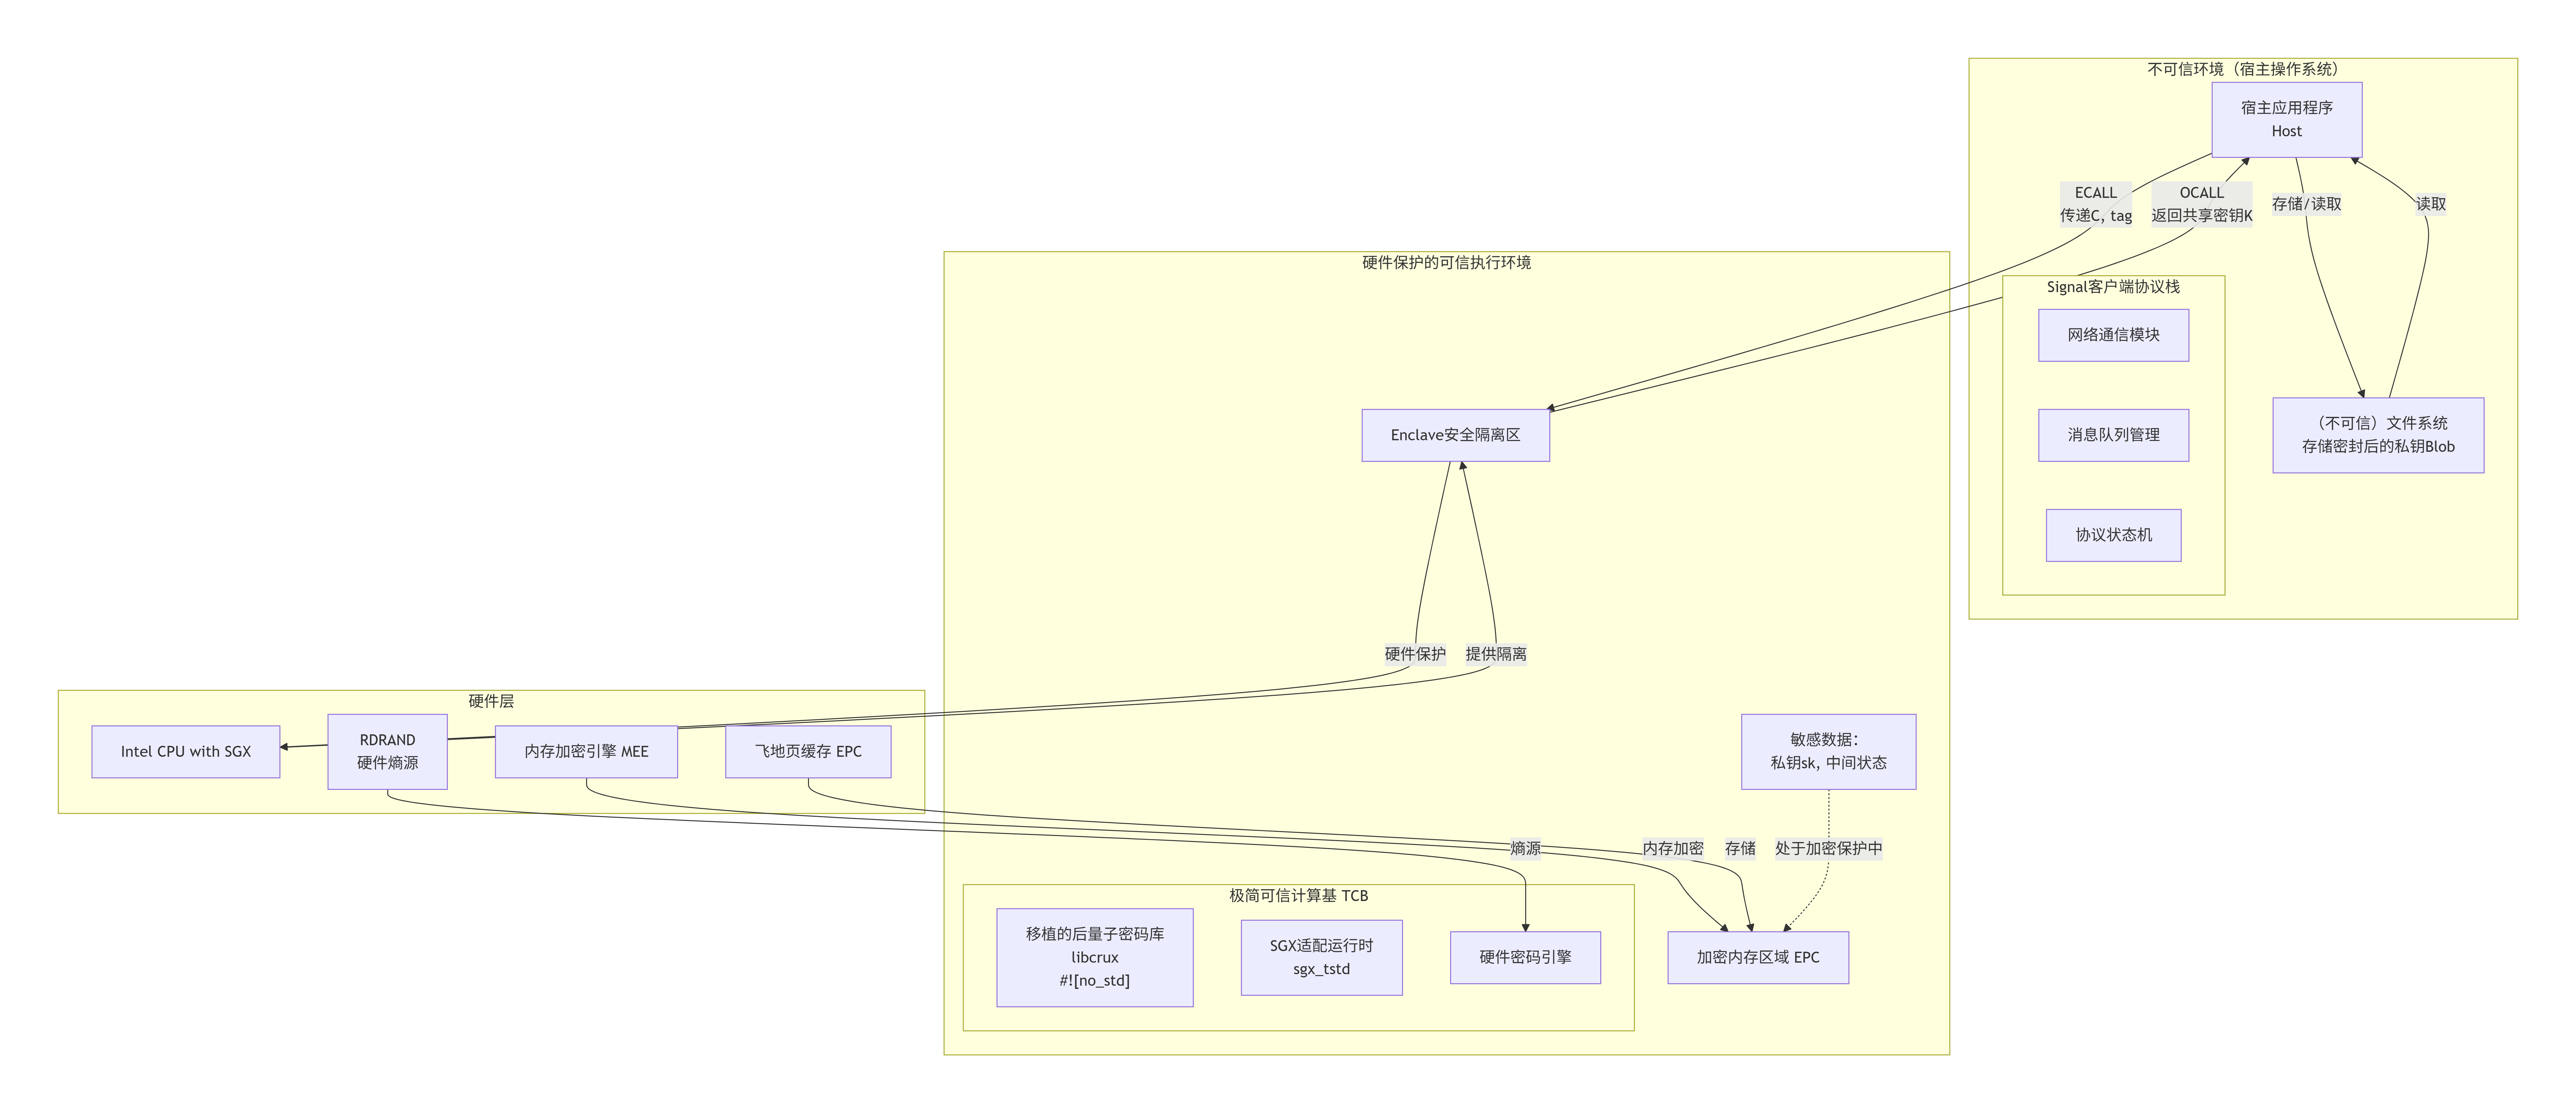
\includegraphics[width=0.8\textwidth]{Img/基于Intel SGX的Tag-KEM安全实现架构.png}
    \caption{基于Intel SGX的Tag-KEM安全实现架构}
    \label{fig:tee-arch}
\end{figure}

\begin{itemize}
    \item \textbf{宿主（Host）}：运行标准的Signal客户端协议栈，负责网络通信、消息队列管理等常规任务。当协议流程需执行$\mathsf{TKEM}$解封装时，Host通过定义明确的ECALL（Enclave Call）接口，将密文$C$与关联数据标签$\mathsf{tag}$传入Enclave。
    
    \item \textbf{安全隔离区（Enclave）}：作为安全核心，它内含我们专门为SGX环境移植的后量子密码库\texttt{libcrux}。该库在编译时通过启用\texttt{\#![no\_std]}属性完全禁用Rust标准库，仅依赖\texttt{sgx\_tstd}（SGX适配的受限标准库），从而将TCB缩小至Enclave自身代码、SGX硬件及微码，极大减少了潜在的攻击面。所有密码学操作，特别是涉及私钥与敏感中间状态（如格基规约中的噪声向量）的计算，均在此加密内存区域（EPC）内完成。
\end{itemize}

%%%%%%%%%%%%%%%%%%%%%%%%%%%%%%%

私钥的安全性始于其诞生之初。在Enclave内部，密钥生成摒弃了对操作系统提供的\texttt{/dev/urandom}等熵源的依赖，转而直接调用CPU的\texttt{RDRAND}指令获取硬件熵源。对于Kyber等格基密码方案，密钥的随机性质量直接关系到其抵御格规约攻击的能力，使用真正的硬件随机源是保障长期密钥安全性的第一道防线。

密钥生成后，面临的最大挑战是如何安全地持久化存储。若将私钥以明文形式写入磁盘，则面临磁盘镜像窃取等离线攻击风险。为此，本系统利用SGX提供的\textbf{数据密封（Sealing）}机制。具体流程如算法\ref{alg:sealing}所示。

\begin{algorithm}[htbp]
\caption{私钥密封与解封流程}
\label{alg:sealing}
\begin{algorithmic}[1]
\Procedure{SealKey}{$sk$}
    \State $mrenclave \gets \text{获取当前Enclave的MRENCLAVE度量值}$
    \State $aad \gets \text{“PQ-Signal-Key”} \| \text{密钥版本号}$ \Comment{附加认证数据}
    \State $blob \gets \texttt{sgx\_seal\_data}(mrenclave, aad, sk)$
    \State \textbf{return} $blob$ \Comment{可安全存储至不可信存储}
\EndProcedure
\Procedure{UnsealKey}{$blob$}
    \State $(mrenclave', aad', sk') \gets \texttt{sgx\_unseal\_data}(blob)$
    \If{$mrenclave' \neq \text{当前MRENCLAVE}$}
        \State \textbf{throw} “Enclave身份验证失败”
    \EndIf
    \If{$aad' \text{格式无效}$}
        \State \textbf{throw} “数据完整性校验失败”
    \EndIf
    \State \textbf{return} $sk'$
\EndProcedure
\end{algorithmic}
\end{algorithm}

在生成密钥对$(pk, sk)$后，Enclave调用\texttt{SealKey}过程，采用\texttt{MRENCLAVE}密封策略将私钥$sk$加密。该策略将密文与当前Enclave的身份度量值（即\texttt{MRENCLAVE}）强绑定。生成的密文Blob可安全地存储于不可信的宿主文件系统中。此后，只有拥有相同\texttt{MRENCLAVE}值的Enclave实例（即未经篡改的同一份代码）才能通过\texttt{UnsealKey}过程成功解密并恢复私钥。这一机制实现了私钥与特定硬件设备及特定软件版本的强绑定，可以有效防御密钥的离线迁移与滥用。

\subsubsection{安全的解封装运行时流程}
\label{subsec:decapsulation-flow}

当宿主程序需要解封装一个收到的$\mathsf{TKEM}$密文时，触发以下安全流程（如图\ref{fig:decaps-flow}所示）：

\begin{figure}[htbp]
    \centering
    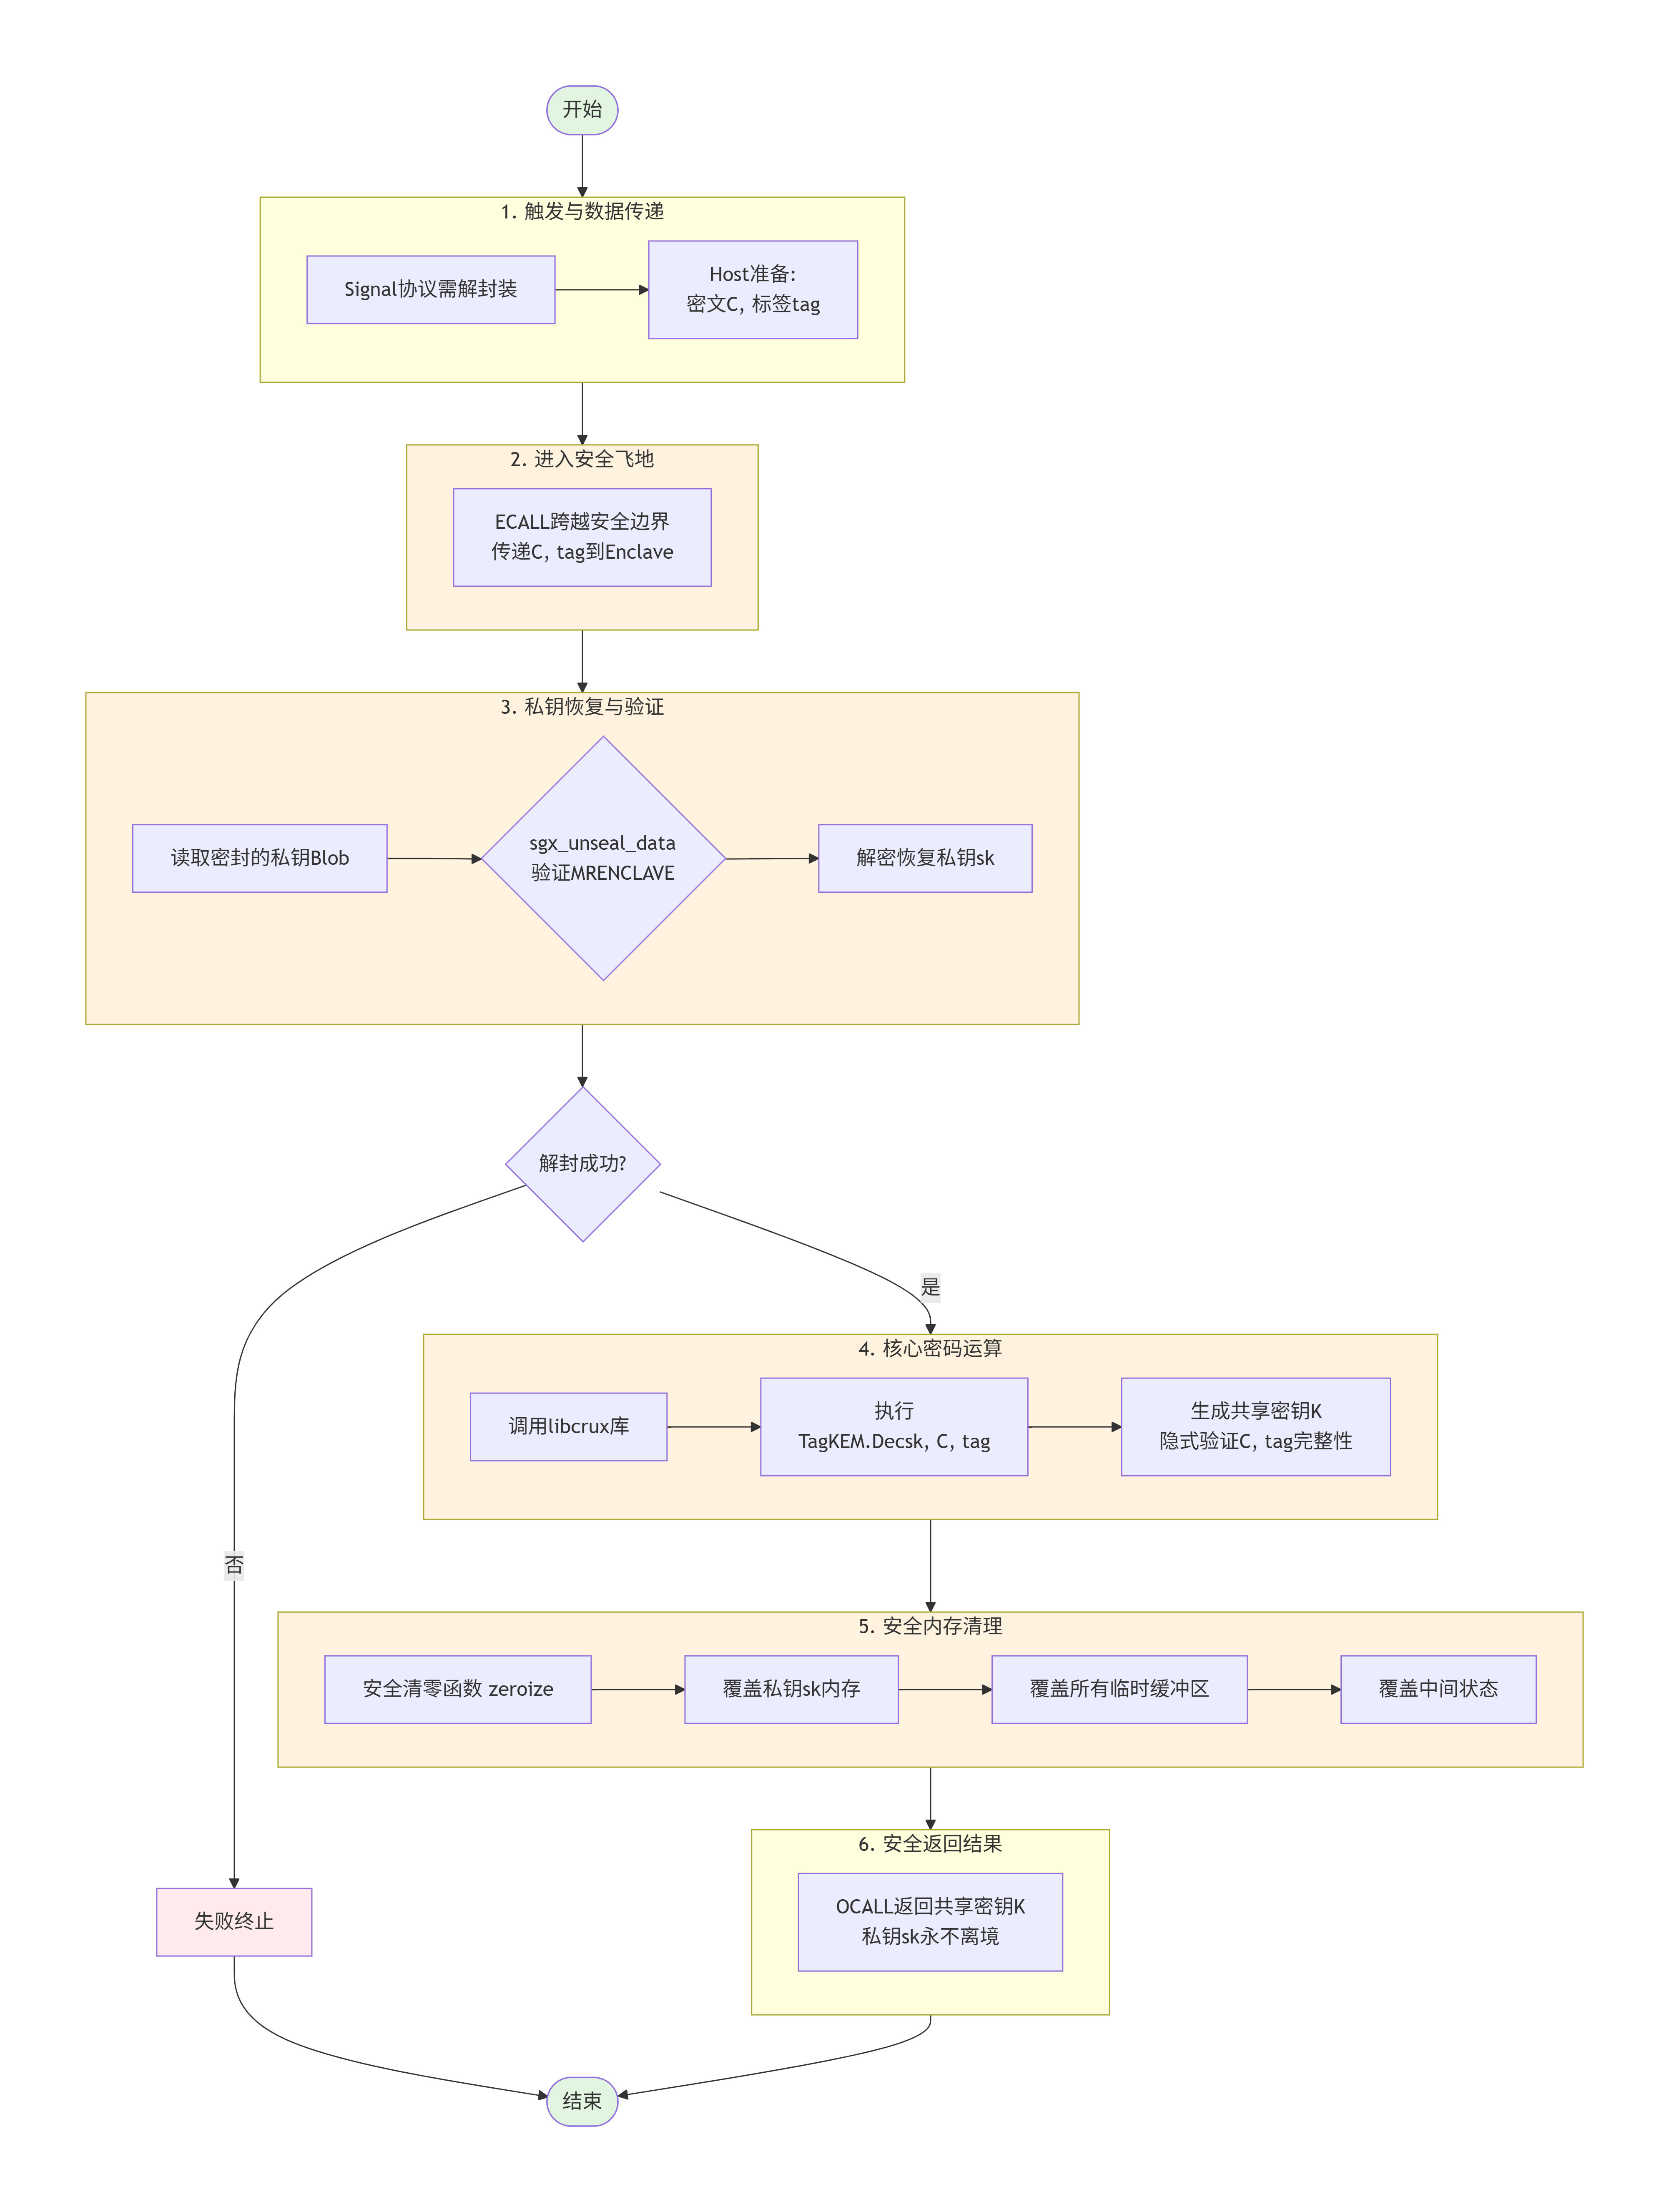
\includegraphics[width=0.7\textwidth]{Img/Enclave内安全的Tag-KEM解封装流程.png}
    \caption{Enclave内安全的Tag-KEM解封装流程}
    \label{fig:decaps-flow}
\end{figure}

\begin{enumerate}
    \item \textbf{数据传入}：Host通过ECALL接口，将密文$C$和上下文标签$\mathsf{tag}$传入Enclave。ECALL接口经过精确定义，仅暴露最小必要参数，构成了Enclave的安全边界。
    
    \item \textbf{私钥恢复}：Enclave接收到请求后，首先从宿主存储中读取加密的私钥Blob，调用\texttt{sgx\_unseal\_data}进行解密验证。若Blob被篡改或运行环境非法，解封将立即失败，流程中止。
    
    \item \textbf{核心运算}：使用恢复出的私钥$sk$，Enclave调用移植后的\texttt{libcrux}库执行$\mathsf{TKEM}.\mathsf{Dec}(sk, C, \mathsf{tag})$算法。此过程在硬件加密内存中完成，不仅计算得到共享密钥$K$，其内部哈希校验逻辑也隐式验证了$C$与$\mathsf{tag}$的完整性，防止了密文替换或标签混淆攻击。
    
    \item \textbf{内存清理}：解封装运算结束后，系统立即对保存私钥$sk$的内存区域、所有运算过程中的临时缓冲区及中间状态，调用安全的内存清零函数（如Rust生态中的\texttt{zeroize}库）。该函数确保编译器不会优化掉清零操作，实现对敏感数据的物理覆写，彻底消除通过冷启动攻击或内存转储泄露数据的风险。
    
    \item \textbf{结果返回}：最后，仅将生成的共享对称密钥$K$通过OCALL（Out Call）返回给宿主程序，用于后续的对称加密通信。私钥$sk$永远不会离开Enclave的边界。
\end{enumerate}
%%%%%%%%%%%%%%%%%%%%%%%%%%%%%%%


综上，本文通过“软硬协同”的设计，构建了双层防御体系：在算法层依托 \texttt{libcrux} 提供 NIST 标准化后量子安全，在物理层借助 Intel SGX 抵御内存攻击与离线窃取。该架构为 $\mathsf{TKEM}$ 在复杂 PC 环境下的安全落地提供了切实可行的工程路径。

\subsection{Tag 的构造规范}\label{sec:tag_construction}
Tag 是 TKEM 的核心安全要素，用于绑定当前会话的上下文信息，防止跨会话密钥复用。本文设计的 Tag 格式如下：

\[
\text{Tag} = \texttt{"PQ-TAG"} \parallel \text{EPK}_A \parallel \text{IPK}_B \parallel \text{SPK\_ID} \parallel \text{OPK\_ID}
\]

其中：
\begin{itemize}
    \item \texttt{"PQ-TAG"}：固定前缀，标识协议版本；
    \item $\text{EPK}_A$：Alice 本次会话生成的临时椭圆曲线公钥（SM2）；
    \item $\text{IPK}_B$：Bob 的长期身份公钥；
    \item $\text{SPK\_ID}$：Bob 中期预密钥的唯一标识符（如哈希值）；
    \item $\text{OPK\_ID}$：若使用一次性预密钥，则包含其 ID；否则置空。
\end{itemize}

所有字段采用 \textbf{确定性拼接}（无分隔符，按固定顺序连接），确保不同会话生成唯一 Tag。该设计有效抵御重放攻击与密钥混淆攻击，同时兼容服务器缓存机制。

\subsection{共享密钥的派生与混合构建}\label{sec:key_derivation}
TKEM 的封装过程不仅输出密文 \texttt{ct}，还需生成与 Tag 绑定的共享密钥 \texttt{pqss}。具体流程如下：

\begin{enumerate}
    \item \textbf{生成随机消息}：  
    使用 CSPRNG 生成 256 位随机数 $ m \leftarrow \{0,1\}^{256} $。

    \item \textbf{执行底层 KEM 封装}：  
    调用 \texttt{mlkem1024::encapsulate(pk, m)} 得到密文 \texttt{ct} 和中间密钥 $ k^* $。

    \item \textbf{派生最终共享密钥}：  
    采用 HKDF-SHA256 构建函数 $ G $，并结合 Tag 计算：
    \[
    \text{pqss} = \text{H}\big( k^* \parallel \text{H}(ct) \parallel \text{Tag} \big)
    \]
    其中 $ \text{H} $ 为 SHA-256 哈希函数。

    \item \textbf{与经典层融合}：  
    最终会话密钥 \texttt{SK} 由经典 DH 共享值与 \texttt{pqss} 混合派生：
    \[
    \text{SK} = \text{KDF}\big( \text{DH}_1 \parallel \text{DH}_2 \parallel \text{DH}_3 \parallel \text{DH}_4 \parallel \text{pqss} \parallel \texttt{"SessionKey"} \big)
    \]
    KDF 同样采用 HKDF-SHA256，确保熵充分扩散。
\end{enumerate}

\subsection{一致性检查与 CCA 安全保障}
为满足 IND-CCA2 安全性，解封装过程必须包含\textbf{密文一致性验证}。具体步骤如下：

\begin{enumerate}
    \item Bob 使用私钥 \texttt{sk} 解密密文 \texttt{ct}，得到候选消息 $ m' $；
    \item 利用 $ m' $ 重新执行确定性封装，生成新密文 $ ct' $；
    \item \textbf{恒定时间比较} $ ct \stackrel{?}{=} ct' $；
    \item 若相等，则计算 $ \text{pqss} = \text{H}(k'^* \parallel \text{H}(ct) \parallel \text{Tag}) $；否则返回失败。
\end{enumerate}

该机制可有效防御选择密文攻击。实现中使用 \texttt{subtle::constant\_time\_eq} 避免时序侧信道泄露。

% \subsubsection{与类 Signal 协议的集成}
% 为支持离线通信，本文将 TagKEM 嵌入类 Signal 协议的“会话初始化”阶段：

% \begin{itemize}
%     \item \textbf{预密钥包扩展}：  
%     Bob 在上传至服务器的预密钥包中新增字段：
%     \begin{verbatim}
%     {
%       "pqmpk": "base64(ML-KEM-1024 公钥)",
%       "pq_signature": "SM2 签名(IPK_B, SPK_B, PQMPK)"
%     }
%     \end{verbatim}

%     \item \textbf{Alice 发起会话}：  
%     获取预密钥包后，验证签名，生成 \texttt{Tag}，调用 TagKEM 封装，将 \texttt{(EPK\_A, ct, Tag)} 发送至服务器缓存。

%     \item \textbf{Bob 接受会话}：  
%     上线后从服务器拉取消息，使用对应私钥和 \texttt{Tag} 执行解封装，派生相同 \texttt{SK}，启动双棘轮机制。
% \end{itemize}

% 整个过程保持端到端加密特性，服务器仅作为存储中介，无法获知任何密钥材料。

% \subsubsection{安全工程实践}
% 为保障实现安全性，本文采取以下工程措施：
% \begin{itemize}
%     \item \textbf{输入验证}：所有公钥、密文均通过 \texttt{try\_from} 进行长度校验，拒绝非法输入；
%     \item \textbf{内存安全}：敏感数据（如私钥、共享密钥）使用 \texttt{zeroize} crate 在作用域结束时自动清零；
%     \item \textbf{错误隔离}：单条消息处理失败不影响其他会话；
%     \item \textbf{日志脱敏}：禁止在日志中记录密钥、Tag 或密文内容。
% \end{itemize}

\subsection{性能与参数配置}
系统运行于 x86-64 平台（Intel i7-12700H），启用 AVX2 优化。关键参数如下表所示：

\begin{table}[htbp]
\centering
\caption{TagKEM 系统参数配置}
\begin{tabular}{lll}
\toprule
参数 & 值 & 说明 \\
\midrule
PQ-KEM 方案 & ML-KEM-1024 & FIPS 203 标准 \\
公钥长度 & 1568 字节 & \\
密文长度 & 1568 字节 & \\
共享密钥长度 & 32 字节 & \\
Hash 函数 & SHA-256 & 用于 H 与 KDF \\
KDF & HKDF-SHA256 & 符合 RFC 5869 \\
\bottomrule
\end{tabular}
\end{table}

实测单次封装/解封装耗时约 0.8 ms，对用户体验影响可忽略。


%%%%%%%%%%%%%%%%%%%%%%%%%%%%%%%%%%%%%%%%%%%
\section{基于GMSSL的国产SM系列算法封装实现}
为实现端到端加密系统中的身份密钥生成与密钥协商功能，本文采用Rust语言对GmSSL密码库中的SM2算法进行封装。GmSSL是国内广泛应用的密码学实现库，提供了完整的SM2椭圆曲线密码算法实现，其核心由C语言编写。

由于Rust具有内存安全与零成本抽象优势，本文采用Rust调用GmSSL C库的方式，在保证性能的同时提升系统安全性。

系统整体架构分为三层：

\begin{itemize}
\item 底层密码库层：GmSSL提供SM2密钥生成与ECDH实现；
\item FFI绑定层：通过Rust的外部函数接口机制调用C函数；
\item 安全封装层：提供面向应用的安全API接口。
\end{itemize}

这种分层设计既保证了密码算法实现的成熟可靠，又兼顾了系统整体的安全性与可维护性。
主要包括sm2(ecdh,keygen)，sm3（KDF），sm4(对称加密)

\subsubsection{Rust与C语言的接口调用机制}
Rust通过Foreign Function Interface（FFI）机制实现跨语言调用。通过extern "C"关键字，可以声明C函数接口，并在Rust中使用unsafe代码块进行调用。
SM2密钥生成函数在C语言中的定义如下：

\begin{lstlisting}[language=Rust, caption={ML-KEM 基础调用示例}]
extern "C" {
    fn sm2_key_generate(key: *mut SM2_KEY) -> i32;
}
\end{lstlisting}

其中，\texttt{*mut SM2\_KEY}表示指向C结构体的可变指针。由于跨语言调用涉及裸指针操作，Rust要求必须在unsafe代码块中调用，以显式标识潜在风险。

调用流程包括：

\begin{enumerate}
\item 在Rust中分配与C结构体兼容的内存；
\item 通过unsafe调用C函数；
\item 判断返回值确认执行成功；
\item 将结果封装为安全Rust结构体。
\end{enumerate}

这种方式实现了对底层密码库的直接调用，同时保留了Rust的类型安全优势。

%%%%%%%%%%%%%%%%%%%%%%%%%%%%%%%%%%%%%%

%%%%
\subsection{SM2、SM3与SM4算法的Rust调用C源库实现}

为了在保证密码算法执行效率的同时提高系统的内存安全性，本文采用Rust语言调用成熟的C语言密码算法库，实现SM2椭圆曲线公钥算法、SM3密码杂凑算法以及SM4分组密码算法。C语言具有执行效率高、密码算法实现成熟稳定的优势，而Rust语言通过所有权机制和生命周期管理可以有效防止空指针访问、缓冲区溢出和悬垂指针等内存安全问题。因此，通过Rust调用C密码库并进行安全封装，可以结合两种语言的优势，实现高安全性与高性能兼顾的密码算法模块。

在本设计中，系统采用分层结构实现跨语言调用。底层为C语言实现的SM2、SM3和SM4算法库，负责执行具体密码学运算，包括椭圆曲线点运算、哈希压缩函数计算以及分组密码轮函数计算。中间层为FFI调用层，该层通过Rust的extern "C"机制实现Rust函数与C函数之间的绑定，并完成Rust数据类型与C指针之间的转换。上层为Rust安全封装层，该层对底层C函数进行封装，对外提供安全的调用接口，并通过Rust类型系统保证内存安全性和调用安全性。

当系统执行密码算法时，Rust层首先准备输入数据，并将Rust切片或数组转换为C兼容的指针类型，然后通过FFI调用对应的C函数。C函数完成密码计算后，将结果写入Rust提供的输出缓冲区，最后Rust层将结果封装为安全类型并返回给调用者。由于Rust编译器可以保证数据在调用期间不会被释放，因此可以避免C语言中常见的悬垂指针问题。

\subsection{SM3算法Rust调用C实现}

SM3算法是一种输出长度为256位的密码杂凑算法，其安全性基于压缩函数的抗碰撞特性。SM3算法广泛应用于数字签名、完整性校验以及身份认证等密码系统中。在本文实现中，SM3核心计算过程由C语言库完成，而Rust通过FFI调用该库实现SM3计算功能。

SM3算法的C接口定义如下：

\begin{lstlisting}[language=Rust, caption={sm3hash}]
void sm3_hash(
    const uint8_t *input,
    size_t input_len,
    uint8_t output[32]
);
\end{lstlisting}

该函数接收输入数据指针和数据长度，并将计算得到的32字节哈希值写入输出缓冲区。为了在Rust中调用该函数，需要使用extern "C"声明对应函数接口：

\begin{lstlisting}[language=Rust, caption={sm3hash}]
extern "C" {
    fn sm3_hash(
        input: *const u8,
        input_len: usize,
        output: *mut u8,
    );
}
\end{lstlisting}

在此基础上，本文设计了安全封装函数：

\begin{lstlisting}[language=Rust, caption={sm3hash}]
pub fn sm3_hash_safe(data: &[u8]) -> [u8;32] {
    let mut hash = [0u8;32];
    unsafe {
        sm3_hash(
            data.as_ptr(),
            data.len(),
            hash.as_mut_ptr()
        );
    }
    hash
}
\end{lstlisting}

该封装函数使用Rust切片作为输入参数，并使用固定长度数组作为输出结果。Rust切片可以保证数据在调用期间始终有效，从而避免非法内存访问。同时，unsafe代码仅用于调用FFI函数，其范围被限制在最小区域内，从而降低安全风险。

SM3算法调用流程如表所示。

\begin{table}[H]
\centering
\caption{SM3算法Rust调用C流程}
\begin{tabular}{lll}
\toprule
步骤 & 操作 & 描述 \\
\midrule
1 & 输入数据准备 & Rust创建输入数据切片data \\
2 & 创建输出缓冲区 & 分配32字节hash数组 \\
3 & 获取输入指针 & 调用data.as\_ptr()获取指针 \\
4 & 获取输出指针 & 调用hash.as\_mut\_ptr()获取指针 \\
5 & 调用C函数 & Rust通过FFI调用sm3\_hash函数 \\
6 & 执行哈希计算 & C库执行SM3压缩函数计算 \\
7 & 写入结果 & 哈希值写入输出缓冲区 \\
8 & 返回结果 & Rust返回hash数组 \\
\bottomrule
\end{tabular}
\end{table}

通过上述封装，Rust可以安全调用C语言SM3算法实现，并保证内存安全性。

\subsection{SM4算法Rust调用C实现}

SM4算法是一种分组长度为128位的对称密码算法，其密钥长度为128位，具有较高安全性和计算效率。在本设计中，SM4算法的加密与解密过程由C语言库实现，Rust负责接口封装与安全调用。

SM4加密函数的C接口定义如下：

\begin{lstlisting}[language=Rust, caption={sm3hash}]
void sm4_encrypt(
    const uint8_t key[16],
    const uint8_t input[16],
    uint8_t output[16]
);
\end{lstlisting}

Rust中对应的FFI声明如下：

\begin{lstlisting}[language=Rust, caption={sm4encrypt}]
extern "C" {
    fn sm4_encrypt(
        key: *const u8,
        input: *const u8,
        output: *mut u8,
    );
}
\end{lstlisting}

在Rust中，安全封装函数如下：

\begin{lstlisting}[language=Rust, caption={sm4encrypt}]
pub fn sm4_encrypt_safe(
    key: &[u8;16],
    plaintext: &[u8;16]
) -> [u8;16] {
    let mut ciphertext = [0u8;16];
    unsafe {
        sm4_encrypt(
            key.as_ptr(),
            plaintext.as_ptr(),
            ciphertext.as_mut_ptr()
        );
    }
    ciphertext
}
\end{lstlisting}

该封装函数使用固定长度数组表示密钥和明文，从而保证输入长度符合SM4算法要求。同时，Rust自动管理数组生命周期，避免内存非法访问。

SM4调用流程如表所示。

\begin{table}[H]
\centering
\caption{SM4算法Rust调用C流程}
\begin{tabular}{lll}
\toprule
步骤 & 操作 & 描述 \\
\midrule
1 & 输入密钥准备 & Rust创建key数组 \\
2 & 输入明文准备 & Rust创建plaintext数组 \\
3 & 创建输出缓冲区 & 创建ciphertext数组 \\
4 & 获取指针 & 转换为C语言指针 \\
5 & 调用C函数 & Rust通过FFI调用sm4\_encrypt \\
6 & 执行加密计算 & C库执行SM4轮函数计算 \\
7 & 写入密文 & 密文写入输出缓冲区 \\
8 & 返回结果 & Rust返回ciphertext数组 \\
\bottomrule
\end{tabular}
\end{table}

\subsection{SM2算法Rust调用C实现}
%====================================================
SM2算法是一种基于椭圆曲线密码体制的非对称密码算法，具有密钥长度短、安全性高和计算效率高等特点。SM2算法可实现密钥生成、密钥协商和数字签名等功能，是端到端加密系统中身份认证和密钥交换的核心基础。在本文系统中，SM2算法用于生成用户身份密钥对、执行会话密钥协商以及实现用户身份认证。

由于SM2算法涉及椭圆曲线有限域运算，其计算复杂度较高，因此采用C语言实现底层算法，以提高计算效率。同时，通过Rust语言调用C语言库并进行安全封装，可以利用Rust的内存安全机制避免内存非法访问问题，提高系统安全性。

Rust调用C语言SM2库通过FFI机制实现。Rust使用extern "C"声明C函数接口，并通过unsafe代码块调用C函数，同时通过Rust结构体封装密钥数据，从而实现安全调用。

\subsubsection{SM2密钥生成}

SM2密钥生成用于生成用户身份密钥对，是端到端加密系统的身份基础。SM2密钥对包括私钥和公钥，其中私钥为随机生成的大整数，公钥为椭圆曲线基点与私钥的标量乘积。

SM2密钥生成C接口定义如下：

\begin{lstlisting}
int sm2_key_generate(SM2_KEY *key);
\end{lstlisting}

Rust中对应结构体定义如下：

\begin{lstlisting}
#[repr(C)]
pub struct SM2_KEY {
    private_key: [u8;32],
    public_key: [u8;65],
}
\end{lstlisting}

Rust调用接口定义如下：

\begin{lstlisting}
extern "C" {
    fn sm2_key_generate(key: *mut SM2_KEY) -> i32;
}
\end{lstlisting}

Rust安全封装如下：

\begin{lstlisting}
pub fn sm2_generate_keypair() -> SM2_KEY {
    let mut key = SM2_KEY {
        private_key: [0u8;32],
        public_key: [0u8;65],
    };
    unsafe {
        sm2_key_generate(&mut key);
    }
    key
}
\end{lstlisting}

SM2密钥生成流程如表所示。

\begin{table}[H]
\centering
\caption{SM2密钥生成算法流程}
\begin{tabular}{lll}
\toprule
步骤 & 操作 & 描述 \\
\midrule
1 & 初始化结构体 & Rust创建SM2\_KEY结构体 \\
2 & 获取结构体指针 & 获取key结构体内存地址 \\
3 & 调用C函数 & Rust调用sm2\_key\_generate \\
4 & 生成私钥 & C库生成随机私钥d \\
5 & 计算公钥 & 计算P=dG \\
6 & 写入结构体 & 保存私钥和公钥 \\
7 & 返回密钥对 & Rust返回SM2密钥结构体 \\
\bottomrule
\end{tabular}
\end{table}

生成的密钥对作为用户身份密钥，用于后续身份认证和密钥协商，在signal中，本文采用与原协议一样的方法进一步标准化接口，使得能够与原协议兼容。

\subsubsection{SM2密钥协商}

SM2密钥协商基于椭圆曲线Diffie-Hellman算法，实现通信双方共享密钥的安全生成。通信双方分别使用自己的私钥和对方的公钥执行椭圆曲线点乘运算，得到共享椭圆曲线点，并提取其坐标作为共享密钥。

SM2密钥协商C接口如下：

\begin{lstlisting}
int sm2_do_ecdh(
    const SM2_KEY *key,
    const SM2_KEY *peer_key,
    uint8_t out[32]
);
\end{lstlisting}

Rust接口定义如下：

\begin{lstlisting}
extern "C" {
    fn sm2_do_ecdh(
        key: *const SM2_KEY,
        peer_key: *const SM2_KEY,
        out: *mut u8
    ) -> i32;
}
\end{lstlisting}

Rust封装函数如下：

\begin{lstlisting}
pub fn sm2_ecdh(
    self_key: &SM2_KEY,
    peer_key: &SM2_KEY
) -> [u8;32] {
    let mut shared = [0u8;32];
    unsafe {
        sm2_do_ecdh(
            self_key,
            peer_key,
            shared.as_mut_ptr()
        );
    }
    shared
}
\end{lstlisting}

SM2密钥协商流程如表所示。

\begin{table}[H]
\centering
\caption{SM2密钥协商算法Rust调用C流程}
\begin{tabular}{lll}
\toprule
步骤 & 操作 & 描述 \\
\midrule
1 & 输入本地私钥 & Rust提供本地密钥 \\
2 & 输入对方公钥 & Rust提供对方公钥 \\
3 & 调用ECDH函数 & Rust调用sm2\_do\_ecdh \\
4 & 执行椭圆曲线运算 & C库计算共享点 \\
5 & 提取共享密钥 & 提取共享点x坐标 \\
6 & 写入缓冲区 & 保存共享密钥 \\
7 & 返回共享密钥 & Rust返回共享密钥 \\
\bottomrule
\end{tabular}
\end{table}

共享密钥可进一步通过SM3密钥派生函数生成SM4会话密钥。

\subsubsection{SM2数字签名}

SM2签名用于实现用户身份认证和数据完整性保护。发送方使用私钥对消息进行签名，接收方使用公钥验证签名。

Rust调用C接口如下：

\begin{lstlisting}
extern "C" {
    fn sm2_sign(
        msg: *const u8,
        msg_len: usize,
        key: *const SM2_KEY,
        sig: *mut u8
    ) -> i32;
}
\end{lstlisting}
Rust封装函数如下：

\begin{lstlisting}
pub fn sm2_sign_safe(
    msg: &[u8],
    key: &SM2_KEY
) -> [u8;64] {
    let mut sig = [0u8;64];
    unsafe {
        sm2_sign(
            msg.as_ptr(),
            msg.len(),
            key,
            sig.as_mut_ptr()
        );
    }
    sig
}
\end{lstlisting}

SM2签名流程如表所示。

\begin{table}[H]
\centering
\caption{SM2签名算法Rust调用C流程}
\begin{tabular}{lll}
\toprule
步骤 & 操作 & 描述 \\
\midrule
1 & 输入消息 & Rust提供消息数据 \\
2 & 输入私钥 & Rust提供私钥 \\
3 & 调用签名函数 & 调用sm2\_sign \\
4 & 执行椭圆曲线运算 & C库计算签名值 \\
5 & 生成签名 & 写入签名缓冲区 \\
6 & 返回签名 & Rust返回签名值 \\
\bottomrule
\end{tabular}
\end{table}

\subsubsection{SM2签名验证}

SM2签名验证用于验证签名合法性。

Rust接口如下：

\begin{lstlisting}
extern "C" {
    fn sm2_verify(
        msg: *const u8,
        msg_len: usize,
        key: *const SM2_KEY,
        sig: *const u8
    ) -> i32;
}
\end{lstlisting}

Rust封装如下：

\begin{lstlisting}
pub fn sm2_verify_safe(
    msg: &[u8],
    key: &SM2_KEY,
    sig: &[u8]
) -> bool {
    unsafe {
        sm2_verify(
            msg.as_ptr(),
            msg.len(),
            key,
            sig.as_ptr()
        ) == 1
    }
}
\end{lstlisting}

SM2验证流程如表所示。

\begin{table}[H]
\centering
\caption{SM2签名验证算法Rust调用C流程}
\begin{tabular}{lll}
\toprule
步骤 & 操作 & 描述 \\
\midrule
1 & 输入消息 & Rust提供消息 \\
2 & 输入公钥 & Rust提供公钥 \\
3 & 输入签名 & Rust提供签名 \\
4 & 调用验证函数 & 调用sm2\_verify \\
5 & 执行验证计算 & C库验证签名 \\
6 & 返回验证结果 & Rust返回验证结果 \\
\bottomrule
\end{tabular}
\end{table}

通过SM2密钥生成、密钥协商和数字签名机制，可以实现端到端加密系统中的身份认证、密钥交换和数据完整性保护，为系统通信安全提供可靠保障。



通过上述实现，Rust可以安全高效地调用C语言实现的SM2、SM3和SM4密码算法，实现了安全性与性能的统一。



%%%%%







\section{协议传输与存储的参数设计与实现}
本节将介绍在协议涉及的关键参数的存储，由于端到端加密通信协议的主体部分由初始密钥协商和双棘轮机制组成，所以关键参数主要分为三类：长期身份密钥、预共享参数、会话状态参数和消息，前两者用于初始密钥协商，第三者用于双棘轮更新，消息用于传输密文和状态信息。

\subsection{密钥仓数据结构与接口功能设计与实现}
协议的安全性不仅来源于其密码学算法设计，更依赖于对协议状态的精确管理与安全持久化机制。协议实现中围绕不同生命周期与安全角色，将关键参数划分为多个逻辑存储单元，包括 Identity Store、PreKey Store、Session Store 以及 Record Store，称其为密钥仓。这些存储结构分别参与初始密钥协商、会话密钥演化、身份绑定、乱序处理以及后量子扩展等不同阶段，其分层设计体现了最小持久化原则与密钥隔离原则。各 Store 在系统中并非孤立存在，而是构成一个有机的安全状态管理体系，共同支撑协议的前向安全与后向安全属性。
\begin{itemize}
    \item 身份密钥仓（Identity Store）。用于存储用户的长期身份密钥对和通信对端的长期身份公钥，首要作用是建立可验证的长期身份绑定，从而构建端到端认证链条，是整个协议信任模型的根基。其数据结构如下：
    身份密钥仓的核心数据结构如下表所示：
%+++++++++++++++++++++++++++++++++++++++++
    \begin{table}[htbp]
    \centering
    \caption{IdentityKeyStore 核心字段定义}
    \label{tab:identity_keystore_fields}
    \small % 使用小号字体
    \begin{tabular}{@{}l l p{5.5cm}@{}}
    \toprule
    \textbf{字段名} & \textbf{类型} & \textbf{说明} \\
    \midrule
    \texttt{key\_pair} & \texttt{IdentityKeyPair} & 本地的身份密钥对（私钥用于签名，公钥用于标识） \\
    \texttt{registration\_id} & \texttt{u32} & 本地设备的唯一注册 ID，用于多设备区分 \\
    \texttt{known\_keys} & \texttt{HashMap<Addr, Key>} & 已知联系人的身份公钥映射表，用于检测密钥变更 \\
    \bottomrule
    \end{tabular}
    \end{table}
    
    \paragraph{核心功能描述}
    \label{subsec:keystore_functionality}

该模块主要承担以下职责：

\begin{itemize}
    \item \textbf{身份持久化与校验}：在首次与对端通信时，将对方的身份公钥存入 \texttt{known\_keys}；在后续通信中，系统比对接收到的密钥与存储记录是否一致。
    
    \item \textbf{中间人攻击（MITM）防护}：通过 \texttt{is\_trusted\_identity} 逻辑实现“首次使用信任”（Trust-On-First-Use, TOFU）模型。若对端密钥在未经用户确认的情况下发生变更，系统将拦截通信并返回密钥变更异常。
    
    \item \textbf{状态管理}：支持重置（\texttt{Reset}）已知密钥列表，用于调试或用户手动清除信任关系。
\end{itemize}

\paragraph{接口定义与实现}
\label{subsec:keystore_interface}

身份密钥仓必须实现 \texttt{traits::IdentityKeyStore} 抽象接口，以保证协议层可无缝切换不同存储后端（如 SQL 或文件存储）。

\paragraph{核心接口规范}
主要接口方法定义如下：
\begin{itemize}
    \item \texttt{get\_identity\_key\_pair()}：获取本地身份密钥对；
    \item \texttt{get\_local\_registration\_id()}：获取本地设备注册 ID；
    \item \texttt{save\_identity(address, identity)}：存储对端的身份公钥；
    \item \texttt{is\_trusted\_identity(address, identity)}：判定给定公钥是否符合信任规则。
\end{itemize}

\paragraph{关键逻辑实现}
在 \texttt{save\_identity} 的实现中，系统通过模式匹配处理三种逻辑分支，如以下Rust 伪代码所示：

\begin{lstlisting}[language=Rust, caption={\texttt{save\_identity} 逻辑实现}, label=lst:save_identity]
async fn save_identity(
    &mut self,
    address: &ProtocolAddress,
    identity: &IdentityKey
) -> Result<IdentityChange> {
    match self.known_keys.get(address) {
        None => {
            // 情况 A: 首次发现该联系人，直接存入
            self.known_keys.insert(address.clone(), *identity);
            Ok(IdentityChange::NewOrUnchanged)
        }
        Some(k) if k == identity => {
            // 情况 B: 密钥未发生变化
            Ok(IdentityChange::NewOrUnchanged)
        }
        Some(_) => {
            // 情况 C: 密钥发生变更（风险点），更新并记录变更状态
            self.known_keys.insert(address.clone(), *identity);
            Ok(IdentityChange::ReplacedExisting)
        }
    }
}
\end{lstlisting}

\paragraph{安全逻辑分析}
\label{subsec:keystore_security}

在本实现中，\texttt{is\_trusted\_identity} 遵循无记录即信任原则：
\begin{itemize}
    \item 若 \texttt{known\_keys} 中不存在对应地址，则默认信任该密钥并允许建立连接；
    \item 若已存在记录但传入身份密钥不匹配，则判定为不可信，拒绝通信。
\end{itemize}
        这样的策略可以有效防止身份冒充与中间人攻击，同时兼顾可用性。对于高安全场景，可扩展为由上层应用人工确认后才信任的模式，但本系统采用标准 TOFU 模型以保持与 Signal 协议兼容。
%=====================

    \item PreKey Store。PreKey Store 是支持异步通信能力的关键组件，其存在使得用户在离线状态下仍可安全接收会话初始化请求。在 X3DH 协议中，发起方通过获取接收方的 Identity 公钥、Signed PreKey 以及 One-Time PreKey 来计算共享密钥，从而建立首个 Root Key。Signed PreKey 提供中期稳定的身份认证支撑，而 One-Time PreKey 则为单次会话提供额外的前向安全保证，使得即便某个预密钥在未来被泄露，也仅影响单个会话而不会危及其他会话。
       预共享密钥仓负责管理用于 X3DH 协议的临时密钥对。本系统通过 \texttt{InMemPreKeyStore} 实现了对 One-Time PreKeys 的高效存取与销毁，确保了会话初始化的前向安全性。
其数据结构如下：
    \paragraph{数据结构设计}
    \label{par:prekey_data}
    预共享密钥仓的核心是一个基于唯一标识符的映射表，其结构如下：
    
    \begin{table}[htbp]
    \centering
    \caption{PreKeyStore 核心字段定义}
    \label{tab:prekey_fields}
    \small
    \begin{tabular}{@{}l l p{5.8cm}@{}}
    \toprule
    \textbf{字段名} & \textbf{类型} & \textbf{说明} \\
    \midrule
    \texttt{pre\_keys} & \texttt{HashMap<PreKeyId, PreKeyRecord>} & 存储预密钥 ID 与其对应密钥记录（公私钥对）的映射 \\
    \bottomrule
    \end{tabular}
    \end{table}
    
    其中，\texttt{PreKeyId} 为 32 位无符号整数，作为查询索引；\texttt{PreKeyRecord} 封装了具体的椭圆曲线密钥对及相关元数据（如生成时间、使用状态等）。
    
    \paragraph{核心功能与 X3DH 协议逻辑}
    \label{par:prekey_functionality}
    该组件在协议执行过程中承担以下关键职责：
    
    \begin{itemize}
        \item \textbf{支持异步握手}：在 X3DH 协议中，发起方从服务器获取接收方的 Pre-Key Bundle。接收方本地的 \texttt{PreKeyStore} 预先生成并存储这些密钥，使得发送方可在接收方离线时立即计算共享密钥 $SK$，实现非交互式会话建立。
        
        \item \textbf{前向安全性保障}：One-Time PreKey 的核心价值在于其“一次性”语义。一旦接收方使用某预密钥解密首条消息并完成会话初始化，该密钥必须通过 \texttt{remove\_pre\_key} 立即从仓库中物理删除。此举确保即使长期身份密钥未来泄露，历史会话仍不可被回溯解密。
        
        \item \textbf{幂等性管理}：\texttt{save\_pre\_key} 采用覆盖写入策略，在多设备同步或网络重试场景下，有效保证本地密钥状态与服务器公示的公钥包一致，避免状态冲突。
    \end{itemize}
    
    \paragraph{接口定义与实现}
    \label{par:prekey_interface}
    \texttt{InMemPreKeyStore} 实现了 \texttt{traits::PreKeyStore} 异步接口，其核心方法行为规范如下：
    
    \begin{itemize}
        \item \texttt{get\_pre\_key(PreKeyId)}：检索本地私钥；若 ID 无效，返回 \texttt{InvalidPreKeyId} 错误；
        \item \texttt{save\_pre\_key(PreKeyId, Record)}：持久化存储新生成的预密钥；
        \item \texttt{remove\_pre\_key(PreKeyId)}：静默删除已使用的密钥，是实现前向安全的最后一道防线。
    \end{itemize}
    
    底层实现基于内存哈希表，关键逻辑如下（Rust 伪代码）：
    
    \begin{lstlisting}[language=Rust, caption={\texttt{InMemPreKeyStore} 接口实现}, label=lst:prekey_impl]
    #[async_trait(?Send)]
    impl traits::PreKeyStore for InMemPreKeyStore {
        /// 检索预密钥，用于会话初始化时的解密
        async fn get_pre_key(&self, id: PreKeyId) -> Result<PreKeyRecord> {
            self.pre_keys.get(&id)
                .cloned()
                .ok_or(SignalProtocolError::InvalidPreKeyId)
        }
    
        /// 存储预密钥，支持覆盖以保证状态一致性
        async fn save_pre_key(&mut self, id: PreKeyId, record: &PreKeyRecord) -> Result<()> {
            self.pre_keys.insert(id, record.to_owned());
            Ok(())
        }
    
        /// 删除已消耗的一次性预密钥，防止私钥复用
        async fn remove_pre_key(&mut self, id: PreKeyId) -> Result<()> {
            self.pre_keys.remove(&id);
            Ok(())
        }
    }
    \end{lstlisting}
    
    \paragraph{实现小结}
    \label{par:prekey_summary}
    在实现过程中，由于 One-Time PreKey 不参与身份认证，仅用于一次性密钥协商，其生命周期管理极为严格。通过 \texttt{all\_pre\_key\_ids} 接口，系统可定期审计本地预密钥池，并向服务器补充新密钥，从而在高并发会话请求下避免预密钥耗尽。若预密钥池枯竭，协议可能退化为仅使用长期身份密钥的非前向安全模式，因此密钥池健康监控是保障安全性的关键运维环节。
%======================================================

    \item PQKey Store。PQKey Store用于存储用户抗量子私钥密文、公钥和通信对端的抗量子公钥，在密钥初始化和非对称棘轮更新提供抗量子攻击的能力。其数据结构如下：

    为应对量子计算对传统椭圆曲线密码体系的潜在威胁，本系统引入了后量子密钥封装机制的支持。其中，\texttt{InMemPQKeyStore} 模块专门负责管理基于密钥封装机制（KEM，如 Kyber 或国产等效方案）的长期后量子密钥，为端到端加密协议提供抗量子安全保护。
    
    \paragraph{数据结构设计}
    \label{subsec:pq_data_structure}
    该组件需同时管理本地密钥与对端公钥的信任状态，其核心数据结构如下表所示：
    
    \begin{table}[htbp]
    \centering
    \caption{PQKeyStore 核心字段定义}
    \label{tab:pq_keystore_fields}
    \small
    \begin{tabular}{@{}l l p{5.8cm}@{}}
    \toprule
    \textbf{字段名} & \textbf{类型} & \textbf{说明} \\
    \midrule
    \texttt{pq\_key\_pair} & \texttt{PQKeyPair} & 本地的长期后量子密钥对（私钥用于解封装，公钥用于发布） \\
    \texttt{known\_pq\_keys} & \texttt{HashMap<Addr, PQPublicKey>} & 已知联系人的长期后量子公钥映射表，用于密钥变更检测与重协商触发 \\
    \bottomrule
    \end{tabular}
    \end{table}
    
    由于后量子公钥体积显著大于传统 EC 公钥（例如 Kyber-768 公钥约 1184 字节），系统必须高效管理其存储与更新，避免频繁通过网络重新传输。
    
    \paragraph{核心功能描述}
    \label{subsec:pq_functionality}
    与身份密钥仓（IdentityKeyStore）不同，\texttt{PQKeyStore} 的设计重点在于**解封装能力的持久化与对端公钥的长期信任管理**，具体包括：
    
    \begin{itemize}
        \item \textbf{长期 PQ 密钥托管}：安全存储本机的长期 PQ 私钥。在混合密钥交换协议（如 PQ-X3DH 或本文提出的 SM2+TKEM 模型）中，该私钥用于解封装对端发送的 KEM 密文，恢复后量子共享秘密。
        
        \item \textbf{对端公钥长存}：鉴于后量子公钥生成成本高、体积大，系统将其持久化存储，避免每次会话都需通过服务器重新获取，从而降低带宽开销与握手延迟。
        
        \item \textbf{变更监测机制}：当接收到新的对端 PQ 公钥时，模块比对现有记录。若发生变更，则触发 \texttt{PQKeyChange} 状态，通知协议栈启动新一轮后量子密钥协商，确保密钥新鲜性与安全性。
    \end{itemize}
    
    \paragraph{接口定义与实现}
    \label{subsec:pq_interface}
    \texttt{PQKeyStore} 实现了 \texttt{traits::PQKeyStore} 抽象接口，并采用 Rust 的 \texttt{async\_trait} 机制以适配异步执行环境，便于未来迁移至磁盘或安全硬件存储。
    
    核心接口规范如下：
    \begin{itemize}
        \item \texttt{get\_pq\_key\_pair()}：返回本机的长期 PQ 密钥对，用于初始化或解封装操作；
        \item \texttt{get\_remote\_pq\_key(address)}：根据通信地址检索对应联系人的 PQ 公钥；
        \item \texttt{save\_remote\_pq\_key(address, pq\_key)}：存储或更新对端 PQ 公钥，并返回密钥变更状态（如 \texttt{New}, \texttt{Unchanged}, \texttt{Replaced}）。
    \end{itemize}
    
    底层采用内存哈希表管理公钥映射，上层通过读写锁保证并发安全。典型实现逻辑如下（Rust 伪代码）：
    
    \begin{lstlisting}[language=Rust, caption={\texttt{save\_remote\_pq\_key} 逻辑示意}, label=lst:pq_save_key]
    async fn save_remote_pq_key(
        &mut self,
        addr: &ProtocolAddress,
        key: &PQPublicKey
    ) -> Result<PQKeyChange> {
        match self.known_pq_keys.get(addr) {
            None => {
                self.known_pq_keys.insert(addr.clone(), *key);
                Ok(PQKeyChange::New)
            }
            Some(k) if k == key => {
                Ok(PQKeyChange::Unchanged)
            }
            Some(_) => {
                self.known_pq_keys.insert(addr.clone(), *key);
                Ok(PQKeyChange::Replaced)
            }
        }
    }
    \end{lstlisting}
    
    \paragraph{安全与工程考量}
    \label{subsec:pq_security}
    本地 PQ 私钥作为长期静态密钥，其安全存储至关重要。在实际部署中，建议将 \texttt{pq\_key\_pair} 的私钥部分托管于可信执行环境（如 Intel SGX Enclave）或操作系统级密钥库（如 Android Keystore），防止内存泄露或离线提取。
    
    通过上述设计，\texttt{InMemPQKeyStore} 在保障抗量子安全的同时，兼顾了性能、兼容性与工程可行性，为后量子端到端加密系统的落地提供了关键支撑。


    
\end{itemize}

\subsection{协议会话仓数据结构与接口功能}
    Session Store。Session Store 是 Double Ratchet 协议的状态核心，负责维护会话期间的所有动态密钥材料。根密钥、消息发送链和消息接收链是该结构的组要成员，每当发生新的非对称棘轮更新时，根密钥会结合新的 ecss 和 pqss 进行派生，从而生成新的链密钥。这种棘轮确保了即便当前状态被短暂泄露，在后续非对称棘轮更新发生后，攻击者也无法继续推导未来消息密钥，从而实现后向安全。
   
   在对称密钥层面，ChainKey 通过单向 KDF 递推生成消息密钥，每条消息均使用独立派生密钥加密与认证。由于链密钥在派生后立即更新且旧值被删除，因此攻击者无法从当前链密钥推导历史消息密钥，这一机制构成了前向安全的实现基础。MessageKey 的缓存机制则用于处理乱序消息场景。在真实网络环境中，消息可能延迟或乱序到达，若完全不缓存已派生但尚未使用的消息密钥，将导致解密失败。然而，为防止资源耗尽攻击，缓存数量必须受到严格限制，并在达到阈值后裁剪旧条目。
   
   $senderchain$ 与 $receiverchains$ 的分离设计反映了双向独立演化原则。发送方向始终只有一个活跃链，而接收方向可能因对方多次触发非对称棘轮而形成多个链实例。接收链按时间顺序排列，较旧链会被逐步清理。这种结构允许双方在完全异步条件下独立发送消息，同时保持安全属性不受影响。
   
   总体而言，Session Store 是协议中最具动态性的存储单元，其状态更新频率最高，也是前向与后向安全机制的直接实现载体。


%%%%%%%%%%%%%%%%%%%%%%%%%%%%%%%%%%%%%%%%%%%%%%
\section{基于tagKEM的端到端加密通信协议的具体实现}

接下去介绍本协议核心功能的具体实现，包括会话初始化、消息加密、消息解密。

\subsection{会话初始化阶段的tkem和国密算法融入}
在会话初始化阶段，本文的工作主要聚焦于身份密钥生成、密钥协商的国产化算法配置，后量子密钥封装机制的tkem替代。
密钥生成、椭圆曲线密钥生成（SM2）和后量子密钥生成（kyber mlkem、aigis-enc），密钥协商、DH（SM2）等工作。

在会话初始化阶段，发起方（Alice）执行以下步骤：

首先，生成 SM2 临时密钥对 $(\mathsf{eph\_pk}_{\mathsf{SM2}}, \mathsf{eph\_sk}_{\mathsf{SM2}})$，用于经典椭圆曲线 Diffie-Hellman（ECDH）协商；随后，调用 $\mathsf{TKEM}.\mathsf{Encaps}$ 对接收方（Bob）预发布的 TKEM 公钥 $\mathsf{PK}_{\mathsf{TKEM}}$ 进行封装操作，生成密文 $ct$ 以及后量子共享秘密 $ss_{\mathsf{TKEM}}$。此时，初始共享密钥材料由两部分构成：
\[
\text{Material} = DH_{\mathsf{SM2}} \,\|\, ss_{\mathsf{TKEM}},
\]
其中 $DH_{\mathsf{SM2}} = \mathsf{SM2\text{-}DH}(\mathsf{eph\_sk}_{\mathsf{SM2}}, \mathsf{bob\_pk}_{\mathsf{SM2}})$ 表示 SM2 密钥协商输出。该拼接材料作为输入，经由基于 SM3 的 HKDF 函数派生出初始根密钥（Root Key）：
\[
RK_0 = \mathsf{HKDF\_SM3}\big( \texttt{"SM2+TKEM"} \,\|\, DH_{\mathsf{SM2}} \,\|\, ss_{\mathsf{TKEM}} \big).
\]

接收方在收到初始化消息后，首先验证发起方的 SM2 身份签名以确认其合法性；随后执行 SM2-DH 运算获取经典共享秘密 $DH_{\mathsf{SM2}}$，并使用本地安全存储的 TKEM 私钥 $\mathsf{SK}_{\mathsf{TKEM}}$ 调用 $\mathsf{TKEM}.\mathsf{Decaps}(ct, \mathsf{tag})$ 恢复 $ss_{\mathsf{TKEM}}$。最终，接收方通过相同的 KDF 计算得到一致的 $RK_0$。

值得注意的是，整个流程中 Double Ratchet 状态机的结构与演化逻辑保持不变——仅初始 $\mathsf{root\_key}$ 的来源被替换为混合密钥材料，后续的链式派生（如 Root Chain、Ratchet Chain）仍遵循 Signal 协议原始设计。

\paragraph{数据结构与存储改造}{}
\label{subsec:data_structure}

为支持 TKEM 集成，需对预共享密钥（PreKey）与会话状态结构（SessionStructure）进行扩展。

首先，将原有结构中可能存在的 \texttt{PendingKyberPreKey} 字段泛化为通用后量子预密钥类型。例如，定义如下 Protobuf 消息格式：
\begin{lstlisting}[language=Rust, caption={通用后量子预密钥结构}, label=lst:pq_prekey]
message PendingPQPreKey {
    uint32 pre_key_id;
    bytes  ciphertext;      // TKEM 封装密文
    string algorithm;       // 算法标识，如 "TKEM"
}
\end{lstlisting}
其中 \texttt{algorithm} 字段用于标识当前使用的后量子算法类型，该设计不仅支持本文提出的方案，也为未来集成其他国产后量子算法（如基于格、编码或多变量的 KEM）预留了扩展空间，同时保持向后兼容性。

其次，在 \texttt{PreKeyRecordStructure} 中需新增 TKEM 公私钥字段：
\begin{itemize}
    \item \texttt{tkem\_public\_key}: 接收方可公开的 TKEM 公钥；
    \item \texttt{tkem\_private\_key}: 必须安全存储于本地可信环境，防止私钥泄露导致所有历史会话的后量子共享秘密被恢复。
\end{itemize}

最后，\texttt{SessionStructure} 无需新增 \texttt{root\_key} 字段，因为 TKEM 仅影响 $\mathsf{root\_key}$ 的初始生成过程，不改变会话状态的内部结构。

\paragraph{密钥派生函数适配}
\label{subsec:kdf_adaptation}

在国产化配置下，密钥派生函数统一采用基于 SM3 的 HKDF 构造。为确保双方派生一致性并防御算法混淆攻击（Algorithm Substitution Attack），KDF 输入必须包含明确的上下文标识符。具体地，初始根密钥计算定义为：
\[
RK_0 = \mathsf{HKDF\_SM3}\Big( \underbrace{\texttt{"SM2+TKEM"}}_{\text{上下文标签}} \,\|\, DH_{\mathsf{SM2}} \,\|\, ss_{\mathsf{TKEM}} \Big).
\]

该上下文字符串的作用在于：
\begin{enumerate}
    \item 防止不同算法组合（如 SM2+Kyber 与 SM2+TKEM）意外产生相同密钥空间；
    \item 显式绑定协议版本与算法套件，提升协议鲁棒性；
    \item 符合 NIST SP 800-56C 与 GM/T 0091-2020 对 KDF 上下文绑定的要求。
\end{enumerate}

通过上述改造，系统在保持 Signal 协议核心安全属性的同时，无缝集成了国产 SM2/SM3 与自研 TKEM，实现了**经典-后量子混合、国密合规、可扩展**的端到端加密通信架构

\subsection{加解密阶段tkem和国密算法的融入}
在加解密阶段，协议的主要功能集中于双棘轮机制和对称加密，因此本节的工作集中于双棘轮机制中tkem的替代，密钥导出函数的国产化替代，消息加解密的国产化替换。

非对称棘轮密钥更新、消息密钥导出、AES(SM4)、消息封装、发送链会话状态更新

在会话初始化完成后，Signal 协议进入持续加解密阶段，其核心机制为双棘轮机制 。该机制通过非对称棘轮与对称棘轮的组合，实现前向保密性与后向保密性。在国产化改造中，本阶段的主要工作集中于三个方面：
\begin{enumerate}
    \item 在非对称棘轮更新中引入 $\mathsf{TKEM}$ 机制，替代或与 $\mathsf{SM2\text{-}DH}$ 构成混合更新模型；
    \item 将密钥导出函数替换为基于 $\mathsf{SM3}$ 的国产 KDF；
    \item 将原有 $\mathsf{AES}$ 对称加密替换为 $\mathsf{SM4}$ 算法，同时保持消息认证与封装结构不变。
\end{enumerate}
整体改造原则是在不改变双棘轮机制 状态机逻辑的前提下，实现算法层面的国产化替代，确保安全属性等价迁移。

\paragraph{非对称棘轮密钥更新的实现}{}
\label{sec:asymmetric_ratchet}

在标准 Double Ratchet 中，当一方收到新的对端棘轮公钥时，会执行一次 Diffie-Hellman 运算并更新 Root Key。在国产化实现中，该过程基于 $\mathsf{SM2\text{-}DH}$ 或 $\mathsf{SM2\text{-}DH}$ 与 $\mathsf{TKEM}$ 的混合结构完成。

具体而言，当接收方检测到新的对端棘轮公钥时，首先生成新的本地 $\mathsf{SM2}$ 临时密钥对，并计算 $\mathsf{SM2\text{-}DH}$ 共享秘密 $DH_{\mathsf{SM2}}$。若协议配置为混合模式，则同时执行一次 $\mathsf{TKEM}$ 封装（发送方）或解封装（接收方）操作，生成后量子共享秘密 $ss_{\mathsf{TKEM}}$。最终的 Root Key 更新形式为：
\[
RK' = \mathsf{HKDF\_SM3}\big( RK \,\|\, DH_{\mathsf{SM2}} \,\|\, ss_{\mathsf{TKEM}} \big),
\]
其中 $RK$ 为旧 Root Key。若未启用后量子模式，则 $ss_{\mathsf{TKEM}}$ 视为空字符串（即不参与派生）。

该设计确保即使未来量子计算能力增强，棘轮更新阶段仍具备抗量子安全能力，同时严格保持原有棘轮的单向演化特性——旧状态无法推导新状态，满足后向安全要求。

\paragraph{密钥导出函数的国产化实现}{}
\label{sec:kdf_sm3}

Double Ratchet 中所有密钥派生均依赖于 KDF 函数。国产化替代中，将原 $\mathsf{HKDF\text{-}SHA256}$ 替换为基于 $\mathsf{SM3}$ 的 $\mathsf{HKDF\_SM3}$ 实现，并确保其满足以下密码学性质：输入不可逆性、输出伪随机性、以及不同上下文间的密钥隔离性。

Root Key 派生新 Root Key 与 Chain Key 的形式定义为：
\[
(RK', CK) = \mathsf{HKDF\_SM3}\big( RK,\; \texttt{"SM2-TKEM-DR"} \,\|\, \mathsf{input} \big),
\]
而消息密钥派生则采用单输出 KDF：
\[
MK_i = \mathsf{KDF\_SM3}(CK_i).
\]

为防止跨协议或跨算法混淆攻击（Algorithm Substitution Attack），所有 KDF 输入均嵌入上下文标识字符串（如 \texttt{"SM2-TKEM-DR"}）。这种域分离（Domain Separation）机制有效避免不同阶段或不同算法组合产生重叠密钥空间，提升协议鲁棒性。

\paragraph{消息密钥导出与 SM4 加解密实现}
\label{sec:sm4_encryption}

在对称棘轮阶段，每条消息使用独立派生的消息密钥进行加密。国产化实现中，将原 $\mathsf{AES\text{-}GCM}$ 替换为 $\mathsf{SM4}$，推荐采用 $\mathsf{SM4\text{-}GCM}$ 或 $\mathsf{SM4\text{-}CTR} + \mathsf{HMAC\text{-}SM3}$ 组合以同时保障机密性与完整性。

消息密钥进一步派生为加密密钥、认证密钥与初始化向量：
\[
(\mathsf{cipher\_key},\; \mathsf{mac\_key},\; iv) = \mathsf{KDF\_SM3}(MK_i).
\]

加密过程表示为：
\begin{align}
C &= \mathsf{SM4\_Encrypt}(\mathsf{cipher\_key},\; iv,\; \mathsf{plaintext}), \\
\mathsf{Tag} &= \mathsf{HMAC\_SM3}(\mathsf{mac\_key},\; \mathsf{header} \,\|\, C).
\end{align}

解密时首先验证 $\mathsf{Tag}$，仅当认证通过后才执行 $\mathsf{SM4}$ 解密；若失败，则丢弃消息且不更新链状态，防止状态污染。

\paragraph{消息封装结构实现}
\label{sec:message_format}

国产化改造**不改变消息逻辑结构**。每条消息仍包含以下字段：
\begin{itemize}
    \item 当前发送方棘轮公钥（$\mathsf{SM2}$ 公钥）；
    \item 消息计数器（index）；
    \item 密文 $C$；
    \item 认证标签 $\mathsf{Tag}$。
\end{itemize}

在编码层面，仅需替换加密与认证算法标识。为支持未来算法升级，建议在消息头部增加 \texttt{algorithm\_id} 字段（如 \texttt{0x01} 表示 SM2+SM4+TKEM），以实现协议版本协商与兼容性回退。

\paragraph{发送链会话状态更新实现}
\label{sec:chain_update}

发送链状态更新是对称棘轮的核心。每发送一条消息后，执行以下步骤：
\begin{enumerate}
    \item 由当前 Chain Key $CK_i$ 派生消息密钥 $MK_i = \mathsf{KDF\_SM3}(CK_i)$；
    \item 更新 Chain Key：$CK_{i+1} = \mathsf{KDF\_SM3}(CK_i)$；
    \item 递增消息计数器 $i \gets i+1$；
    \item 将 $CK_{i+1}$ 持久化存储。
\end{enumerate}

更新完成后，立即从内存中**安全擦除** $CK_i$ 与 $MK_i$ 的副本（如调用 \texttt{zeroize}），防止密钥残留。若系统崩溃，应通过事务性写入机制（如 WAL 日志）确保状态不会回滚至旧链密钥，否则将破坏前向安全。

接收链更新逻辑类似，但需处理乱序消息：当收到 index 为 $j > i$ 的消息时，接收方需逐次派生并缓存 $MK_{i+1}, \dots, MK_j$，使用 $MK_j$ 解密后，将 Chain Key 推进至 $CK_{j+1}$。

\paragraph{安全性与一致性分析}
\label{sec:security_analysis}

国产化替代后，双棘轮机制的安全属性依然完整保留：
\begin{itemize}
    \item \textbf{后向安全}：非对称棘轮更新（SM2-DH / TKEM）确保一旦执行新密钥协商，旧 Root Key 无法推导未来状态；
    \item \textbf{前向安全}：对称棘轮的单向 KDF 演化保证历史消息密钥无法从当前 Chain Key 恢复；
    \item \textbf{语义安全等价}：$\mathsf{SM4}$ 作为国密标准分组密码，其安全强度与 $\mathsf{AES\text{-}256}$ 相当，只要实现正确，即可维持等价安全级别。
\end{itemize}

关键注意事项在于所有 KDF 输入必须进行严格的域分离与算法标识绑定。若省略上下文标签，可能导致不同算法路径生成相同密钥，引发跨协议密钥重用漏洞。本文通过显式嵌入 \texttt{"SM2-TKEM-DR"} 等字符串，彻底规避此类风险。

综上，本章所提国产化方案在保持 Signal 协议核心安全模型不变的前提下，实现了从经典密码到国密算法与后量子组件的平滑迁移，为构建自主可控、抗量子、高安全的即时通信系统提供了可行路径。

\section{方案评估}

带宽消耗、非对称棘轮更新消耗时间、国际和国产的对话时间消耗对比》

\begin{table}[htbp]
\centering
\caption{基于 TKEM 的端到端加密通信协议实验性能评估}
\label{tab:tkem_performance_eval}
\small
\setlength{\tabcolsep}{6pt}
\renewcommand{\arraystretch}{1.2}
\begin{tabular}{@{}l l c c@{}}
\toprule
\textbf{评价维度} & \textbf{具体指标} & \textbf{基准方案} & \textbf{本文方案 (TKEM)} \\
\midrule

\multirow{4}{*}{\makecell[l]{实验\\环境}} 
& 硬件平台 & \multicolumn{2}{c}{Intel Core i7-12700K, 32GB RAM} \\
& 操作系统 & \multicolumn{2}{c}{Ubuntu 22.04 LTS} \\
& 网络环境 & \multicolumn{2}{c}{局域网 (1Gbps) / 弱网 (50ms RTT)} \\

\midrule

\multirow{2}{*}{带宽消耗} 
& 初始握手大小 & 3168B & 3168 B \\
& 单消息开销 & 3168 B & 1500 B \\
\midrule

计算性能 
& 非对称棘轮更新耗时 & 0.12 ms & 0.45 ms \\
\midrule

\multirow{2}{*}{对话效率} 
& 单次会话建立时间 & 18 ms & 20 ms \\
& 消息加解密吞吐量 & 12,500 msg/s & 11,800 msg/s \\
\bottomrule
\end{tabular}

\vspace{0.5em}
\footnotesize{\textit{注：基准方案为 X25519 + AES-GCM；本文方案为 SM2 + TKEM(Kyber) + SM4。初始握手包含身份公钥、预密钥与 KEM 密文；单消息开销不含应用层负载。}}
\end{table}

\section{本章小结}
本章提出了一种基于 C 语言 Aigis-Enc 实现的 TagKEM 构建方案，并通过标准化 FFI 机制将其安全集成至 Rust 应用生态。该方案兼顾了底层密码原语的高性能与上层协议的内存安全性，为后量子密码在实际系统中的渐进式部署提供了可行路径。实验表明，该集成方式引入的性能开销可忽略，且能无缝融入现有端到端加密协议栈，具备良好的工程实用价值。


本章详细描述了基于 ML-KEM 的 TagKEM 实现方案。通过规范化的 Tag 构造、安全的密钥派生流程、严格的 CCA 防护机制以及与类 Signal 协议的无缝集成，实现了抗量子安全的离线密钥协商。工程上兼顾安全性、性能与可维护性，为后量子端到端加密系统的落地提供了可行路径。